% ====================================================================
% VİZE RAPOR ŞABLONU – Türk Masalları Derlemesi Web Sayfası
% --------------------------------------------------------------------
% DERLEME: Overleaf'te Menu > Compiler > XeLaTeX (pdfLaTeX de çalışır).
%
% KURALLAR (şablonu kullanmadan önce okuyun):
%  1. Bölüm başlıklarını SİLMEYİN ve sırasını DEĞİŞTİRMEYİN.
%  2. [KÖŞELİ PARANTEZ] içindeki ve gri renkli açıklama metinlerini
%     kendi bilgilerinizle değiştirin; açıklama metinlerini silin.
%  3. MEBİS'e YALNIZCA bu raporun PDF'ini yükleyin.
%     ZIP ve HTML dosyası YÜKLEMEYİN. Tüm kontroller GitHub'dan yapılır.
%  4. Kapaktaki GitHub ve YouTube bağlantıları doğru ve tıklanabilir
%     olmalıdır. Teslimden önce PDF'teki bağlantılara tıklayıp deneyin.
%  5. Haftalık katkı tablosundaki görseller için resim dosyalarını
%     (hafta1.png, hafta2.png, ...) Overleaf projesine yükleyin.
%     Dosya adlarında boşluk ve Türkçe karakter kullanmayın.
%     Resim yoksa tabloda "görsel ekleyin" kutusu görünür.
%  6. Yapay zekâ kullandıysanız Bölüm 5'i doldurun.
% ====================================================================
\documentclass[12pt,a4paper]{article}

\usepackage{iftex}
\ifPDFTeX
  \usepackage[T1]{fontenc}
  \usepackage[utf8]{inputenc}
\else
  \usepackage{fontspec}
\fi
\usepackage[turkish]{babel}
\usepackage[margin=2.4cm]{geometry}
\usepackage{setspace}
\usepackage{graphicx}
\usepackage{booktabs}
\usepackage{longtable}
\usepackage{array}
\usepackage{colortbl}
\usepackage{xcolor}
\usepackage{enumitem}
\usepackage{listings}
\usepackage{amssymb}
\usepackage{caption}
\usepackage{fancyhdr}
\usepackage{hyperref}

\onehalfspacing
\setlength{\parindent}{0pt}
\setlength{\parskip}{6pt}
\setlist{itemsep=2pt, topsep=4pt}
\hypersetup{colorlinks=true, linkcolor=blue!50!black, urlcolor=blue!50!black}

\definecolor{ana}{HTML}{14325C}
\definecolor{acik}{HTML}{EEF2F8}

\lstset{basicstyle=\ttfamily\small, backgroundcolor=\color{acik},
  frame=single, rulecolor=\color{ana}, breaklines=true,
  columns=fullflexible, keepspaces=true, showstringspaces=false}

\pagestyle{fancy}
\fancyhf{}
\fancyhead[L]{Masal Bahçesi}
\fancyhead[R]{Vize Raporu}
\fancyfoot[C]{\thepage}

% ---------- Yardımcı komutlar ----------
% Gri açıklama metni (silinecek yönergeler için)
\newcommand{\aciklama}[1]{{\color{gray}\itshape (#1)}}

% Haftalık tablo görseli: dosya yoksa "görsel ekleyin" kutusu çıkar
\newcommand{\haftagorsel}[1]{%
  \IfFileExists{#1}{%
    \includegraphics[width=\linewidth,height=4.2cm,keepaspectratio]{#1}%
  }{%
    \fbox{\parbox[c][2.6cm][c]{\dimexpr\linewidth-2\fboxsep-2\fboxrule\relax}{%
      \centering\small\color{gray} Ekran görüntüsü / görsel ekleyin\\ \texttt{#1}}}%
  }%
}
% Haftalık katılım kutuları (işaretlemek için $\square$ yerine $\boxtimes$ yazın)
\newcommand{\katilimkutulari}{\par\vspace{3pt}\small $\square$ Ders içinde katılım sergiledim\par $\square$ Telafi yaptım}

% Ek görsel: dosya yoksa hiçbir şey göstermez
\newcommand{\haftaek}[1]{%
  \IfFileExists{#1}{\\[4pt]\includegraphics[width=\linewidth,height=4.2cm,keepaspectratio]{#1}}{}%
}

% ---------- Kapak bilgileri ----------
\newcommand{\universite}{Medipol Üniversitesi / Görsel İletişim Tasarımı}
\newcommand{\dersadi}{Programlamaya Giriş}
\newcommand{\hocaadi}{Meral Şentürk}
\newcommand{\ogrenciadi}{Melis Ertaş}
\newcommand{\ogrencino}{86250005}
\newcommand{\projeadi}{Masal Bahçesi}
% Bağlantıları tam adres olarak yazın (https:// ile başlayarak)
\newcommand{\githublink}{\url{https://github.com/melisertas2804-tech/masal-bahcesi}}
\newcommand{\youtubelink}{\url{https://www.youtube.com/watch?v=kvkJe2wEb3k}}

\begin{document}

% ====================================================================
% KAPAK
% ====================================================================
\begin{titlepage}
\centering
\vspace*{1cm}
{\large \universite \par}
\vspace{1.8cm}
{\Huge\bfseries\color{ana} \projeadi \par}
\vspace{0.4cm}
{\Large Türk Masalları Derlemesi Web Sayfası \par}
{\large Vize Raporu \par}
\vspace{1.8cm}
{\large \textbf{Ders:} \dersadi \par}
{\large \textbf{Öğretim Üyesi:} \hocaadi \par}
\vspace{1.2cm}
{\large \textbf{Hazırlayan:} \ogrenciadi \par}
{\large \textbf{Öğrenci No:} \ogrencino \par}
\vspace{1.8cm}
\fbox{\parbox{0.88\linewidth}{\centering\vspace{6pt}
{\large\bfseries Proje Bağlantıları}\\[8pt]
\textbf{GitHub deposu:}\\ \githublink \\[8pt]
\textbf{YouTube sunum videosu:}\\ \youtubelink
\vspace{6pt}}}
\vfill
{\large \today \par}
\end{titlepage}

\tableofcontents
\newpage

% ====================================================================
\section{Giriş}
% ====================================================================
Bu projede, Türk halk anlatı geleneğinden seçtiğim sekiz masalı bir araya getiren Masal Bahçesi adlı web sayfasını hazırladım. Amacım, eski anlatıları günümüz okuru için kolay bulunan ve rahat okunan bir arayüzde sunmaktı. Sayfa, 8--12 masal koşuluna uygun olarak sekiz masal içerir ve tek bir HTML dosyasından oluşur. Stil kodları \texttt{<style>}, betik kodları ise \texttt{<script>} etiketleri içinde yer alır; harici CSS, JavaScript, yazı tipi veya görsel dosyası kullanılmaz. Bu nedenle sayfa internet bağlantısı olmadan da açılıp çalışır. JavaScript; arama, tür filtresi, yazı boyutu ayarı, favoriler ve menü takibi gibi işlevleri yerine getirir. Bu rapor sırasıyla masal seçimini, tasarım kararlarını, kodun çalışma mantığını, yapay zekâ kullanımını, haftalık katkıları ve test sonuçlarını anlatır.

\subsection{Proje Özeti}
Masal Bahçesi; Kültür Portalı'ndaki kaynaklardan yararlanılarak günümüz Türkçesine uyarlanan sekiz masalı suluboya görünümlü görsellerle sunan, tek sayfalık ve çevrimdışı çalışan bir derlemedir. Okur masalları ada veya türe göre bulabilir, yazı boyutunu ayarlayabilir ve sevdiği masalları favorilerine ekleyebilir.

\subsection{Gereksinimlerin Karşılanması}
\begin{center}
\rowcolors{2}{acik}{white}
\begin{tabular}{@{}p{8.2cm}c@{}}
\toprule
\rowcolor{ana}\textcolor{white}{\textbf{Gereksinim}} & \textcolor{white}{\textbf{Durum}} \\
\midrule
Masal sayısı 8--12 arasında (8 masal)         & $\boxtimes$ \\
Tek HTML dosyası                                    & $\boxtimes$ \\
Stil kodları içsel (\texttt{<style>} içinde)        & $\boxtimes$ \\
Betik kodları içsel (\texttt{<script>} içinde)      & $\boxtimes$ \\
İnternetsiz açılıp çalışıyor                        & $\boxtimes$ \\
JavaScript sayfada anlamlı bir işlev görüyor        & $\boxtimes$ \\
Sayfa telefonda da düzgün görünüyor                 & $\boxtimes$ \\
\bottomrule
\end{tabular}
\end{center}
% ====================================================================
\section{Masalların Seçimi}
% ====================================================================
Masalları seçerken öncelikle sayfadaki tür filtresinin gerçekten işe yaramasını istedim, bu yüzden hayvan masalı, öğüt masalı, olağanüstü masal ve halk hikâyesinden örnekler aldım. Ekranda rahatça okunabilmeleri için 232 ile 463 kelime arasında, kısa sürede bitirilebilen metinleri tercih ettim. Seçkinin kendini tekrar etmemesi için her masalın farklı bir temayı işlemesine dikkat ettim. Metinlerin doğrulanabilir olması için de resmî bir kaynak olan T.C. Kültür Portalı'ndan yararlandım.

\begin{longtable}{@{}cp{4cm}p{3cm}p{5.4cm}@{}}
\toprule
\textbf{No} & \textbf{Masal} & \textbf{Tür} & \textbf{Seçilme nedeni} \\
\midrule
\endhead
1 & Felek & Halk hikâyesi & Seçkiye masalın dışında bir halk hikâyesi kattığı ve sadakat temasını mizahla işlediği için seçtim. \\
2 & Üç Haylaz Masalı & Hayvan masalı & Hayvan karakterleriyle çocuk okura yakın duran bu macera, düşünmeden karar vermenin sonuçlarını eğlenceli biçimde gösteriyor. \\
3 & Derviş & Öğüt masalı & Seçkinin 232 kelimelik en kısa metni olan bu masal, öğüt türünü tek cümlelik açık bir mesajla örnekliyor. \\
4 & İncili Çadır & Olağanüstü masal & Padişahı, uzun yolculuğu ve olağanüstü olaylarıyla klasik masal kalıbını temsil eden bu metin, seçkinin de en uzunu. \\
5 & Öksüz Kız & Olağanüstü masal & Üvey anne ve konuşan inek motifleriyle okurun tanıdığı bir masal kalıbının Anadolu'daki örneğini sunuyor. \\
6 & Kurnaz Kurt Masalı & Hayvan masalı & Köylülerle kurdun pazarlığı üzerinden kurnazlık ve korkuyu işlediği için diğer hayvan masallarından daha gerilimli bir ton katıyor. \\
7 & Dört Öğüt & Öğüt masalı & Her öğüdün olaylarla sınandığı kurgusu, sabır ve bilgelik temasını anlatıyla göstermeyi sağlıyor. \\
8 & İnatçı Horoz & Hayvan masalı & Tekrarlı ve zincirleme anlatımıyla sözlü geleneğin yapısını yansıtıyor, sesli okumaya da çok uygun. \\
\bottomrule
\end{longtable}

% ====================================================================
\section{Tasarım Kararları}
% ====================================================================
\subsection{Konuya Uygunluk}
Sayfanın görsel dilini eski bir masal kitabı hissi üzerine kurdum. Giriş görselindeki Anadolu köyü, açık kitap ve fener ile masal kapaklarındaki suluboya sahneler anlatıların geçtiği dünyayı doğrudan yansıtıyor. Kâğıdı andıran krem (\texttt{\#FCF7F1}) sayfa zemini ve bej alanlar kitap duygusunu, morun ve gül renginin birlikte kullanımı ise görsellerdeki gece göğünü ve çiçekleri destekliyor. Başlıklarda ve masal metninde kullandığım tırnaklı yazı tipi de basılı kitap okuma alışkanlığını çağrıştırıyor.

\subsection{Renk Paleti ve Yazı Tipi}
\begin{center}
\rowcolors{2}{acik}{white}
\begin{tabular}{@{}llp{6.4cm}@{}}
\toprule
\rowcolor{ana}\textcolor{white}{\textbf{Ad}} & \textcolor{white}{\textbf{Kod}} & \textcolor{white}{\textbf{Nerede / neden kullandınız?}} \\
\midrule
\relax Mor & \texttt{\#6E4D7D} & Metin, ana düğme ve çizgiler. Krem zeminde 6,53:1 karşıtlık sağladığı için uzun okumaya uygun. \\
\relax Gül & \texttt{\#C97A80} & Vurgu rengi: etiketler, aktif menü ve ``OKU'' bağlantıları. Yalnızca küçük alanlarda kullanılıyor. \\
\relax Bej & \texttt{\#EEDFD2} & Giriş alanı ve Hakkında bölümü. Sayfanın bölümlerini birbirinden ayırıyor. \\
\relax Georgia, Arial & -- & Başlık ve masal metninde kitap hissi veren Georgia, menü ve düğmelerde küçük boyutta net okunan Arial. İkisi de sistem yazı tipi olduğu için internet gerektirmiyor. \\
\bottomrule
\end{tabular}
\end{center}

\subsection{Okunabilirlik, Gezinme ve Duyarlı Tasarım}
\begin{itemize}
  \item \textbf{Okunabilirlik:} Masal metni bilgisayarda 19, telefonda 18 pikseldir; satır aralığı sırasıyla 1,85 ve 1,74'tür. Metin sütunu en fazla 685 pikseldir ve bir satıra yaklaşık 85 karakter sığar. Metin ile zemin arasındaki karşıtlık 6,53:1'dir. Gül rengi krem zeminde 3,0:1, bej zeminde 2,45:1'de kaldığı için bu rengi uzun metinlerde kullanmadım.
  \item \textbf{Gezinme:} Üst menü dört bölüme bağlanır ve bulunulan bölümü gösterir. Masallar kartlar hâlinde listelenir; okur arama yapabilir veya dört tür filtresinden birini seçebilir. Okuma alanındaki ``Masal listesine dön'' ve ``Sıradaki masal'' bağlantıları geçişi kolaylaştırır.
  \item \textbf{Duyarlı tasarım:} Masal kartları bilgisayarda üç, 980 pikselin altında iki sütundur; 360 pikselin altında tek sütuna iner. Giriş alanında görsel üstte, yazılar altta durur ve görsel kırpılmadan tam görünür. 650 pikselin altında menü tüm genişliğe yayılır. Telefonda menü, filtre, kalp ve yazı boyutu düğmelerinin dokunma alanı en az 44 pikseldir. Arama kutusu 16 piksel olduğu için iPhone dokununca sayfayı yakınlaştırmaz.
  \item \textbf{Tutarlılık:} Renkler CSS değişkenlerinden gelir; bu nedenle tüm bölümlerde aynı dört ton kullanılır. Bölüm başlıkları aynı düzeni, kartlar da aynı yapıyı tekrarlar.
\end{itemize}

\subsection{Ekran Görüntüleri}
\begin{figure}[h]
  \centering
  \shorthandoff{=}
  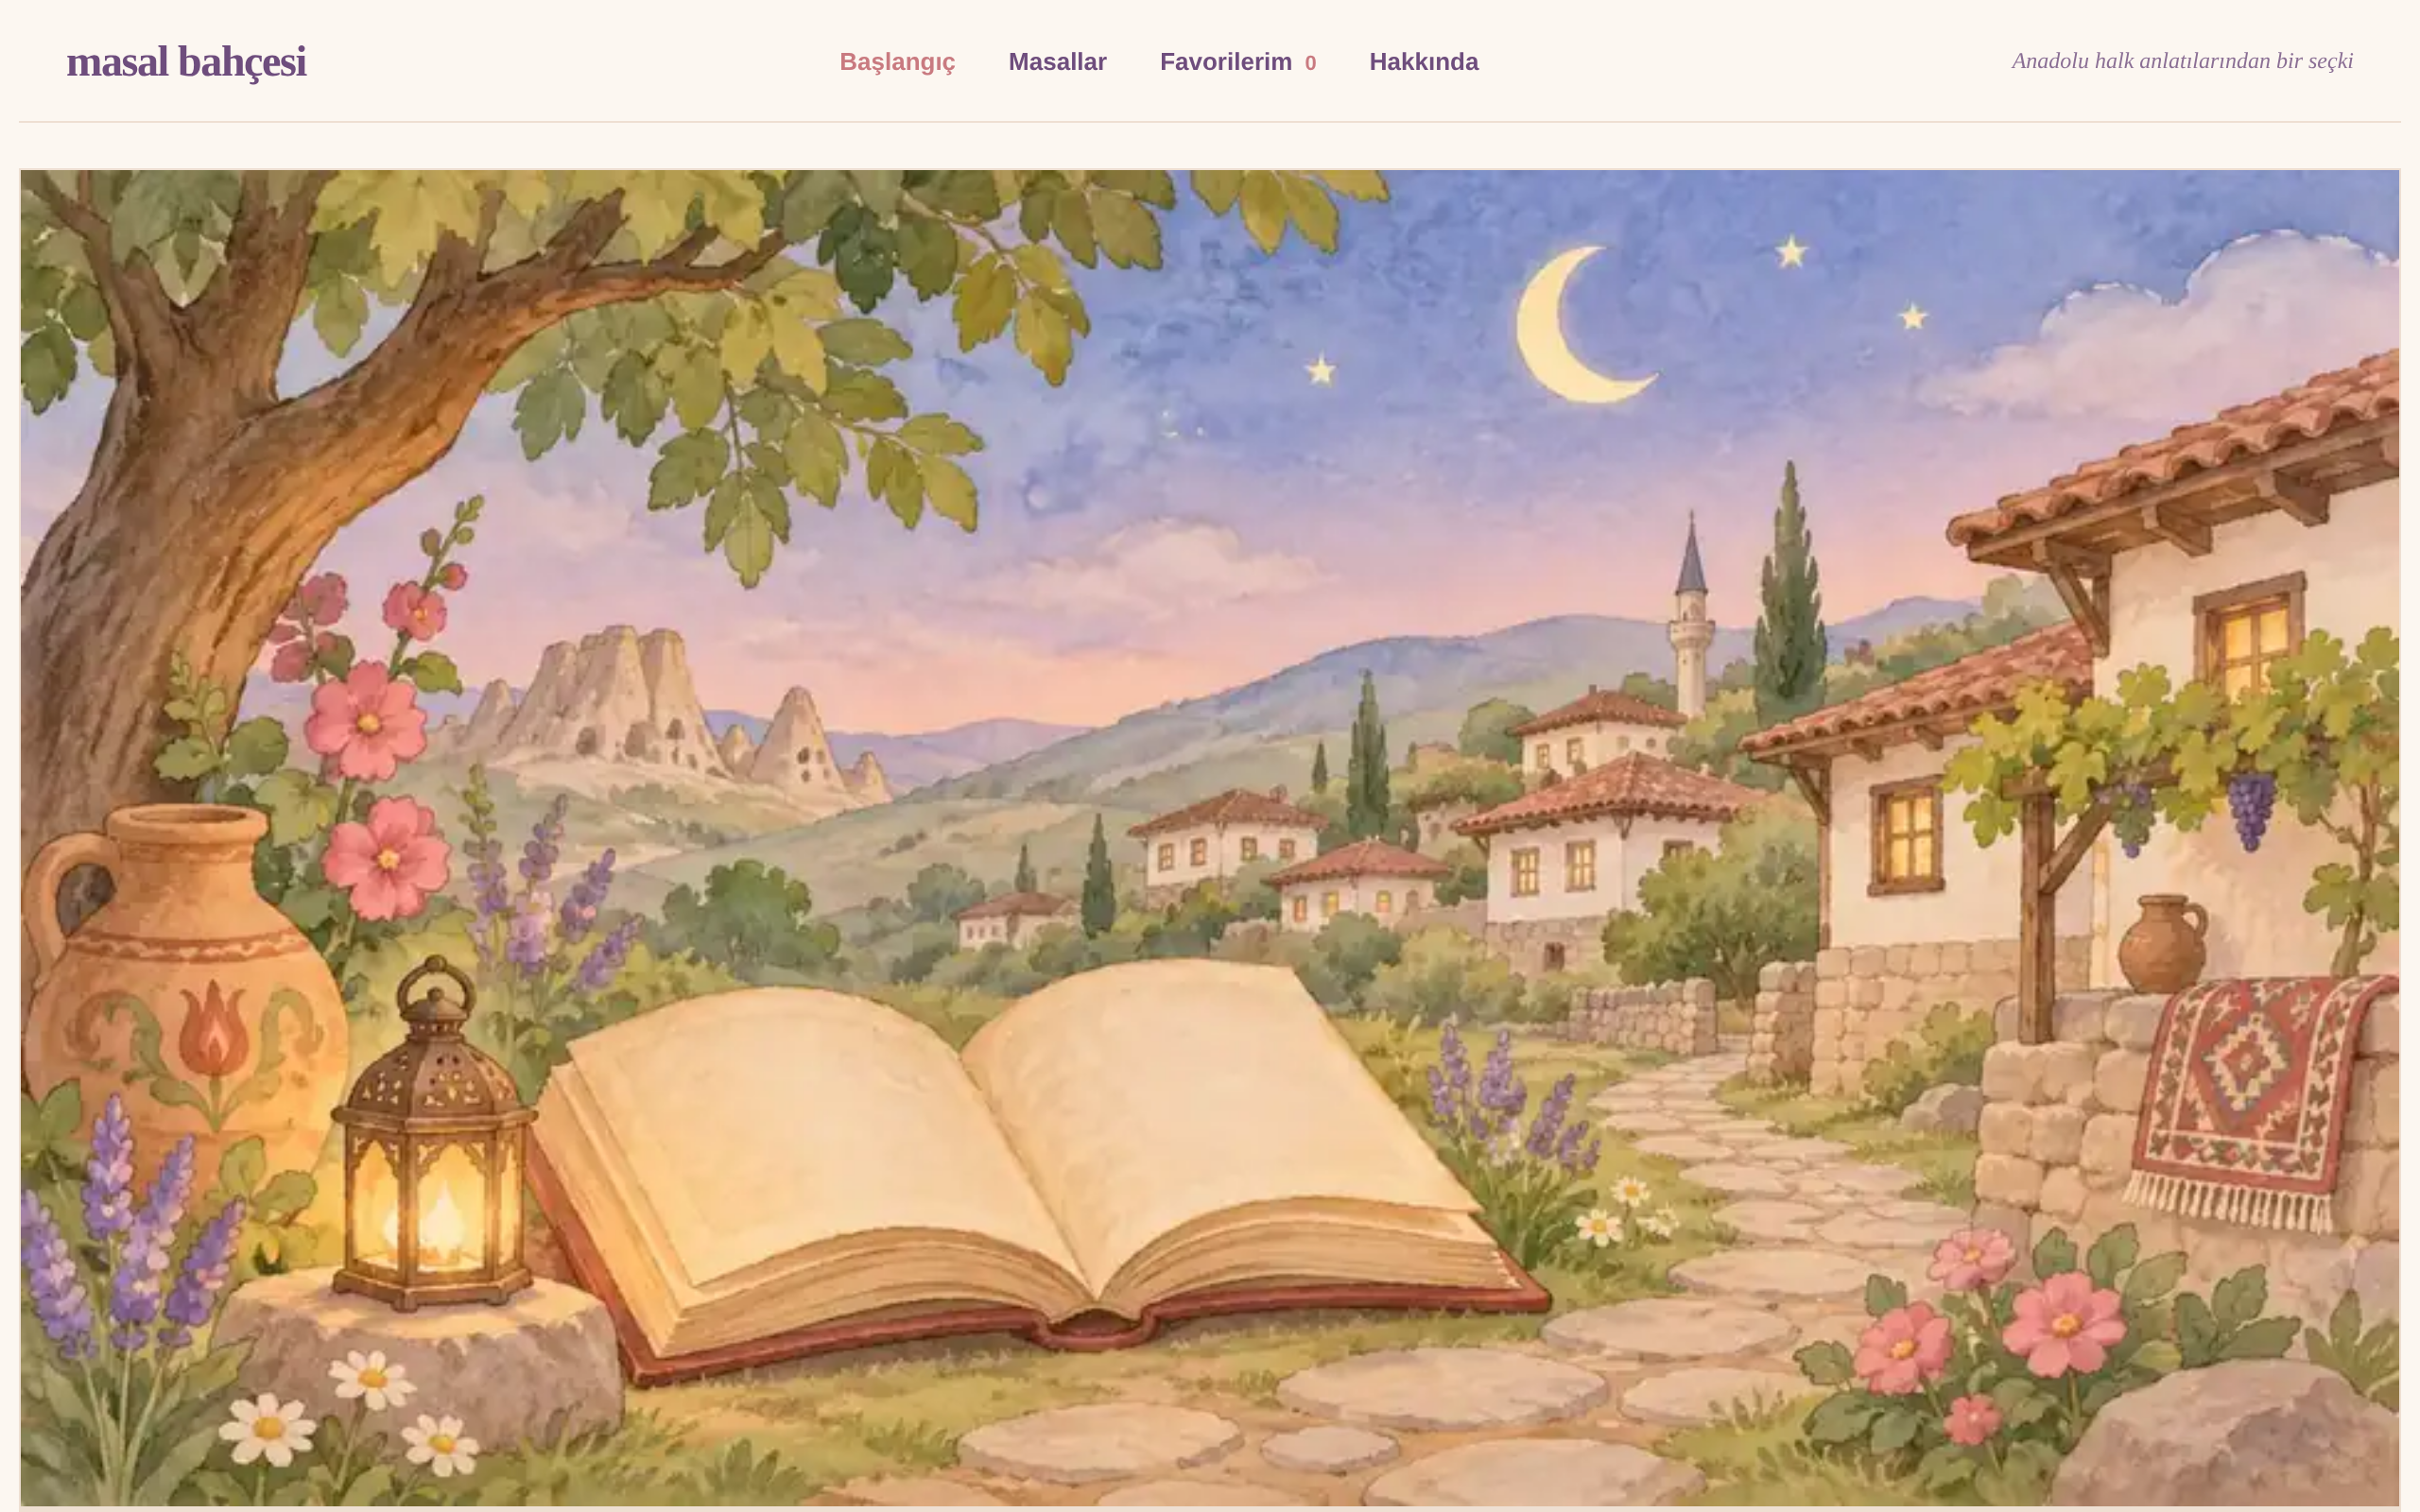
\includegraphics[width=0.9\textwidth]{ekran-masaustu.png}
  \caption{Sayfanın bilgisayar görünümü}
\end{figure}
\begin{figure}[h]
  \centering
  \shorthandoff{=}
  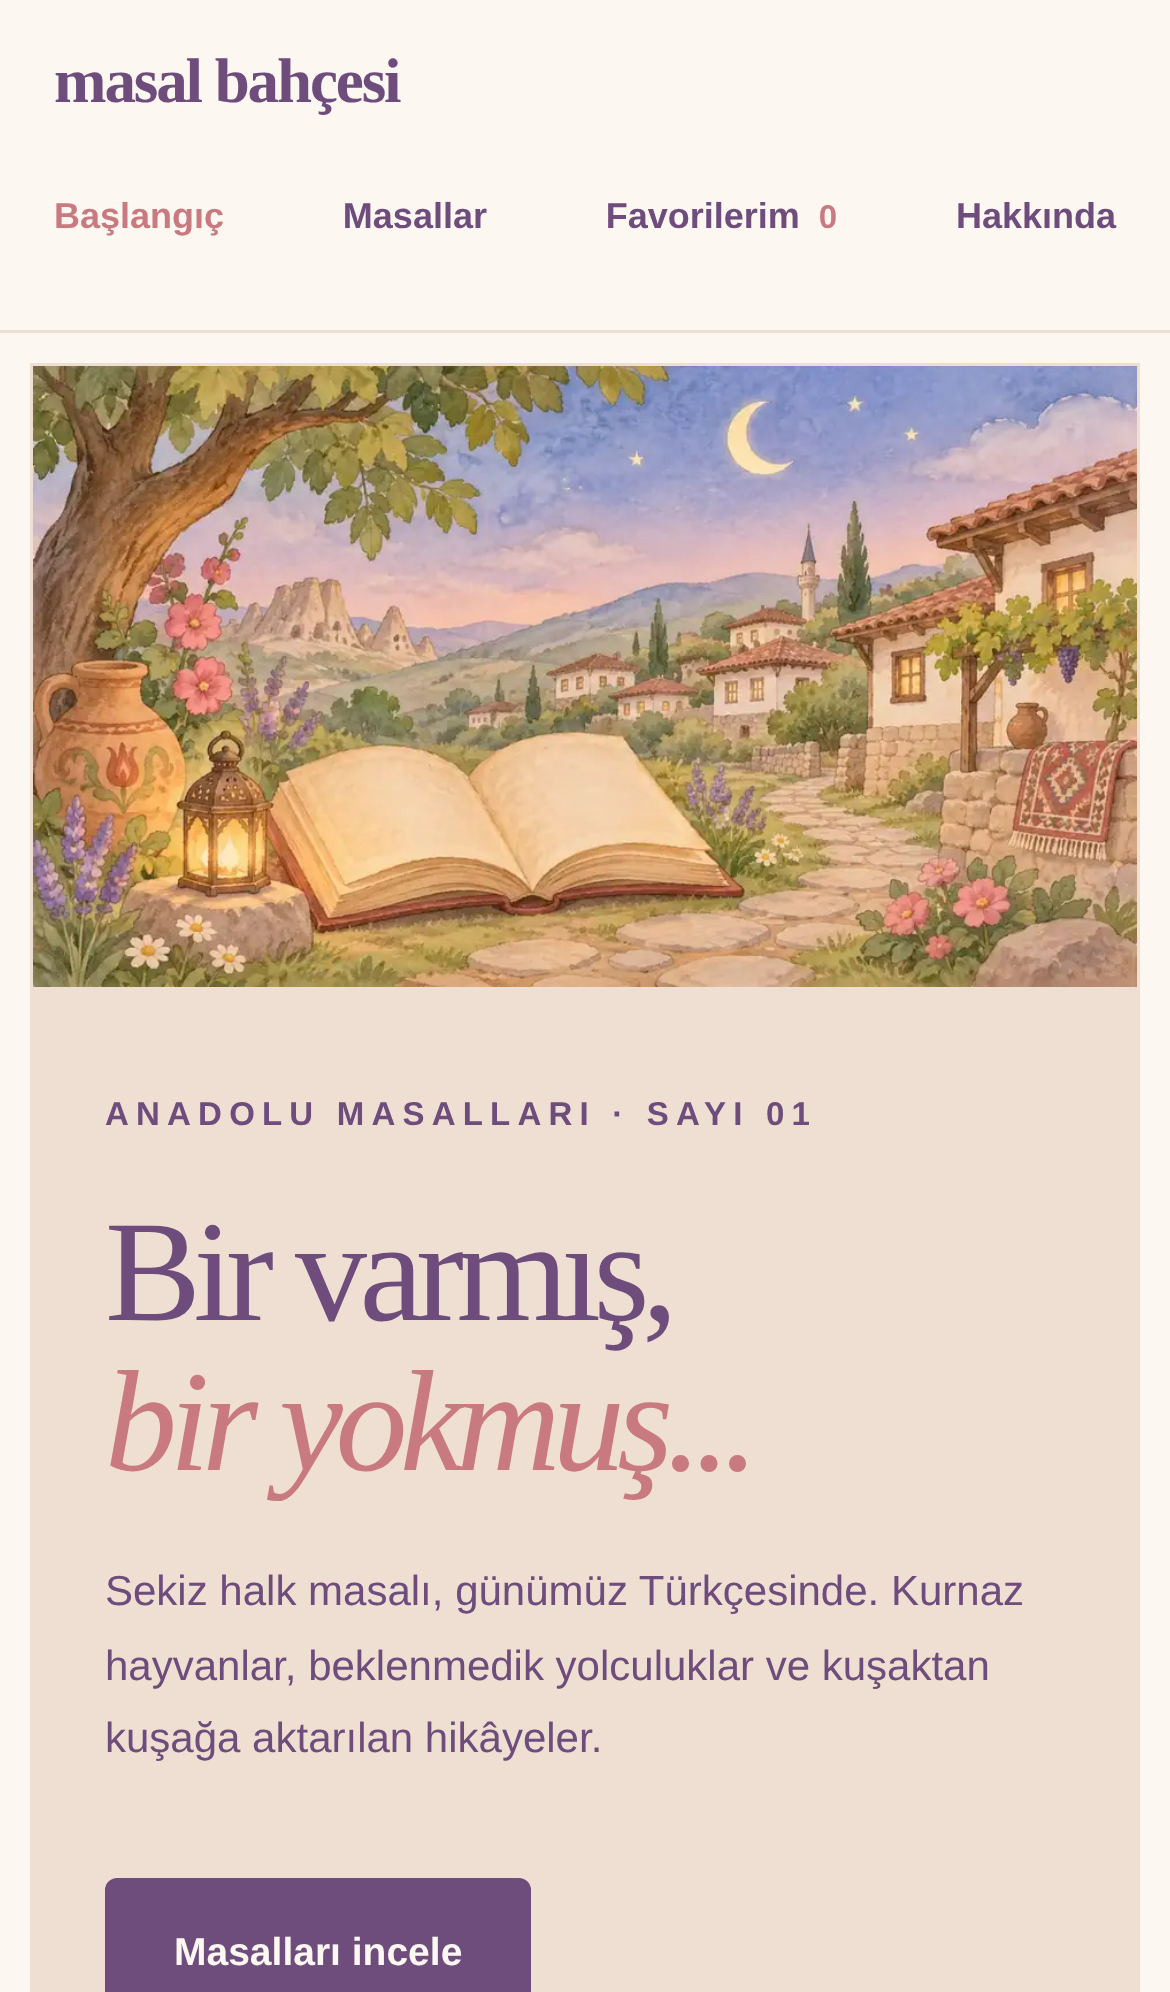
\includegraphics[width=0.35\textwidth]{ekran-mobil.png}
  \caption{Sayfanın telefon görünümü}
\end{figure}

% ====================================================================
\section{Gerçekleştirme}
% ====================================================================
\subsection{HTML Yapısı}
Sayfa sırasıyla üst menü (\texttt{header}, \texttt{nav}), giriş alanı, masal kataloğu, favoriler, masal metinleri, koleksiyon notu (\texttt{section}) ve alt bilgiden (\texttt{footer}) oluşur. Her masal bir \texttt{section} içinde, metni ise \texttt{article} içinde yer alır. Kartlar her masalın kendi adresine bağlantı verir; CSS'teki \texttt{:target} seçicisi yalnızca adresi seçilen masalı görünür yapar. Bu yüzden masallar JavaScript kapalıyken de açılır.

\subsection{İçsel CSS}
Renkleri \texttt{:root} içinde değişken olarak tanımladım. Kart listesinde \texttt{grid}, menü ve araç çubuğunda \texttt{flex} kullandım. Duyarlı tasarım için 980, 650 ve 360 piksellik \texttt{@media} kuralları yazdım. Kapak görselleri dosya içine gömülüdür ve \texttt{background-size: cover} ile kutuyu doldurur.

\begin{lstlisting}[caption={İçsel CSS'ten önemli bir bölüm}]
:root {
  --morc: #6E4D7D;
  --gul: #C97A80;
  --bej: #EEDFD2;
  --krem: #FCF7F1;
}

.kartlar {
  display: grid;
  grid-template-columns: repeat(3, minmax(0, 1fr));
  column-gap: 30px;
  row-gap: 42px;
}
\end{lstlisting}

\subsection{İçsel JavaScript}
Masal verisi ayrı bir JavaScript dizisinde değil, doğrudan HTML'de tutulur. Kartların \texttt{data-tur} ve \texttt{data-arama} öznitelikleri arama ve filtre için kullanılır. \texttt{kartlariSuz()} her kartın seçili türe ve aranan kelimeye uyup uymadığına bakar, uymayanları gizler ve masal sayısını günceller. \texttt{favorileriYukle()} ve \texttt{favorileriKaydet()} favorileri \texttt{localStorage} ile saklar. Aşağıdaki \texttt{favoriKartlariniCiz()} ise favori masalların kartlarını kopyalayıp favoriler bölümüne ekler. \texttt{menuyuGuncelle()} bulunulan bölüme göre menüdeki aktif bağlantıyı değiştirir. Olaylar \texttt{addEventListener} ile bağlanır: arama kutusunda \texttt{input}, düğmelerde \texttt{click}, sayfada \texttt{scroll} ve \texttt{hashchange} dinlenir.

\begin{lstlisting}[caption={İçsel JavaScript'ten önemli bir bölüm}]
function favoriKartlariniCiz() {
  const alan = document.getElementById('favori-kartlar');
  alan.innerHTML = '';

  kartKutulari.forEach(function (kutu) {
    if (!favoriler.has(kutu.dataset.masal)) return;
    const kopya = kutu.cloneNode(true);
    kopya.hidden = false;
    alan.appendChild(kopya);
  });

  alan.hidden = favoriler.size === 0;
  document.getElementById('favori-bos').hidden = favoriler.size !== 0;
}
\end{lstlisting}

\subsection{Sayfanın Özellikleri}
Sayfada masal adı ve içeriğine göre anlık arama, türe göre filtreleme ve görünen masal sayısı bulunur. Okur masalları favorilerine ekleyebilir; favoriler aynı tarayıcıda saklanır. Okuma alanında yazı boyutu 15--29 piksel arasında ayarlanabilir, sıradaki masala ve listeye geçilebilir. Menü bulunulan bölümü gösterir, sayfa başlığı açılan masala göre değişir. Zorlayıcı olay içeren masallarda okur notu yer alır. Düzen telefon ve bilgisayara uyumludur ve sayfa internetsiz çalışır.


% ====================================================================
\section{Yapay Zekâ Kullanımı}
% ====================================================================
\begin{longtable}{@{}p{2.6cm}p{3.6cm}p{4.2cm}p{3.4cm}@{}}
\toprule
\textbf{Araç} & \textbf{Ne için kullandınız?} & \textbf{İstem (prompt) özeti} & \textbf{Sayfada nerede?} \\
\midrule
\endhead
\relax Claude (Anthropic) & Kod ve rapor taslağı & Kodun düzenlenmesi, hataların bulunup düzeltilmesi; rapor metni için taslak hazırlanması. & HTML/CSS/JS yapısı; tür filtresi, menü takibi, favori düğmesi, okur notları, telefon düzeni \\
\relax ChatGPT (OpenAI) & Görsel & Suluboya masal sahneleri; ör. Anadolu köyü, açık masal kitabı ve fener. & Giriş görseli ve sekiz masal kapağı \\
\bottomrule
\end{longtable}

\subsection{Anladığım ve Kendim Yaptığım Kısımlar}
Kodun düzenlenmesi, filtre ve menü gibi hataların giderilmesi ve telefon görünümünün iyileştirilmesinde Claude'dan yardım aldım. Rapor metni için de taslak desteği aldım. Yapay zekâya masal metinlerini ve görselleri değiştirmemesini, raporda şablonun düzenine dokunmamasını söyleyerek sınırları ben belirledim. Önerilen düzeltmeleri okuyup hangilerinin uygulanacağına karar verdim. Sunumda anlatabilmek için kodun bölümlerini, özellikle arama, filtre, favoriler ve menü takibini tek tek inceledim.

% ====================================================================
\section{Haftalık Katkılar}
% ====================================================================
\begin{longtable}{@{}>{\raggedright\arraybackslash}p{1.7cm}%
                    >{\raggedright\arraybackslash}p{6.4cm}%
                    >{\centering\arraybackslash}p{6cm}@{}}
\toprule
\rowcolor{ana}\textcolor{white}{\textbf{Hafta}} & \textcolor{white}{\textbf{Yapılan çalışma}} & \textcolor{white}{\textbf{Görsel}} \\
\midrule
\endfirsthead
\toprule
\rowcolor{ana}\textcolor{white}{\textbf{Hafta}} & \textcolor{white}{\textbf{Yapılan çalışma}} & \textcolor{white}{\textbf{Görsel}} \\
\midrule
\endhead
\bottomrule
\endfoot

\textbf{1. hafta}\newline [tarih] &
Bu hafta derste katılım gerektiren bir çalışma yapılmadı.\newline \textbf{Commit:} --\katilimkutulari &
-- \\
\midrule
\textbf{2. hafta}\newline [tarih] &
WorldWideWeb konulu örnek bir sayfa hazırladım. Başlık, paragraf ve liste etiketlerini kullandım, \texttt{<ul>} içindeki bağlantılarla sayfa içinde gezinmeyi sağladım. \texttt{<style>} içinde gövde, başlık ve bağlantı stillerini yazdım.\newline \textbf{Commit:} 2. hafta: WorldWideWeb sayfasi\par\vspace{3pt}\small $\boxtimes$ Ders içinde katılım sergiledim\par $\square$ Telafi yaptım &
Görsel aşağıda \\*
\multicolumn{3}{c}{\resizebox{12cm}{!}{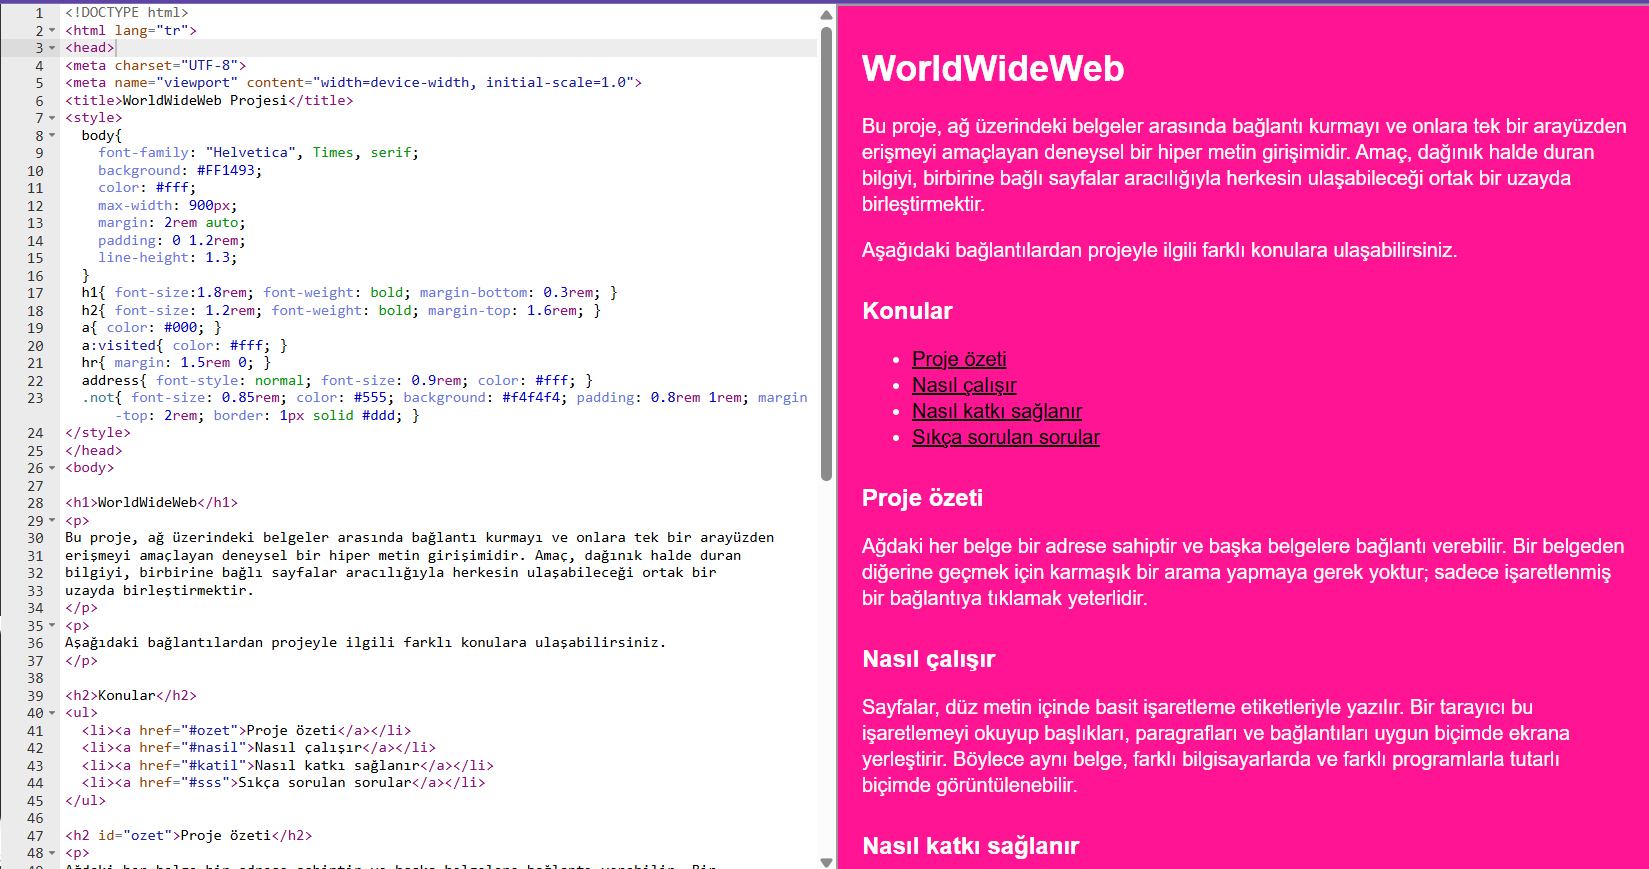
\includegraphics{hafta2.png}}} \\
\midrule
\textbf{3. hafta}\newline [tarih] &
Bu haftayı sonradan telafi ederek tamamladım. \texttt{onclick} ve \texttt{alert} ile indirim kodu örneğini, \texttt{window.open} ile yeni sekme açmayı, \texttt{mouseover} ve \texttt{mouseout} ile renk değiştirmeyi denedim. Adventure Time konulu sayfada \texttt{<style>} ile stil verme, \texttt{<details>} ile açılır liste ve sayfa içi bağlantılar üzerinde çalıştım.\newline \textbf{Commit:} 3. hafta telafi: alert, yeni sekme, mouseover ve Adventure Time\par\vspace{3pt}\small $\square$ Ders içinde katılım sergiledim\par $\boxtimes$ Telafi yaptım &
Görsel aşağıda \\*
\multicolumn{3}{c}{\resizebox{14cm}{!}{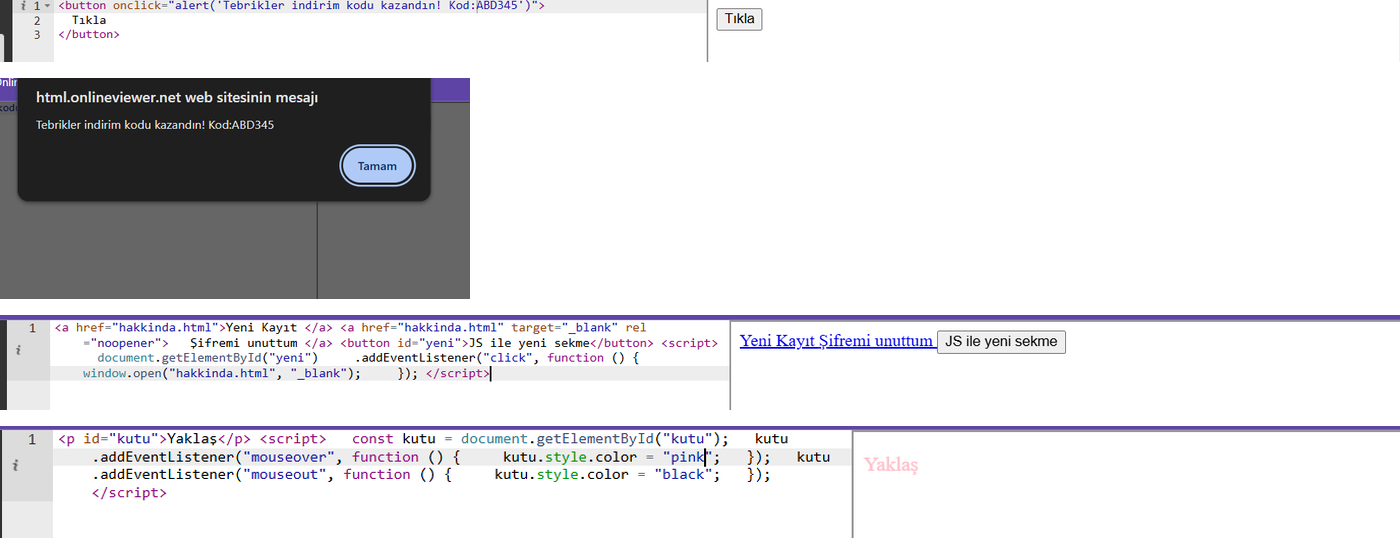
\includegraphics{hafta3.png}}} \\
\multicolumn{3}{c}{\resizebox{14cm}{!}{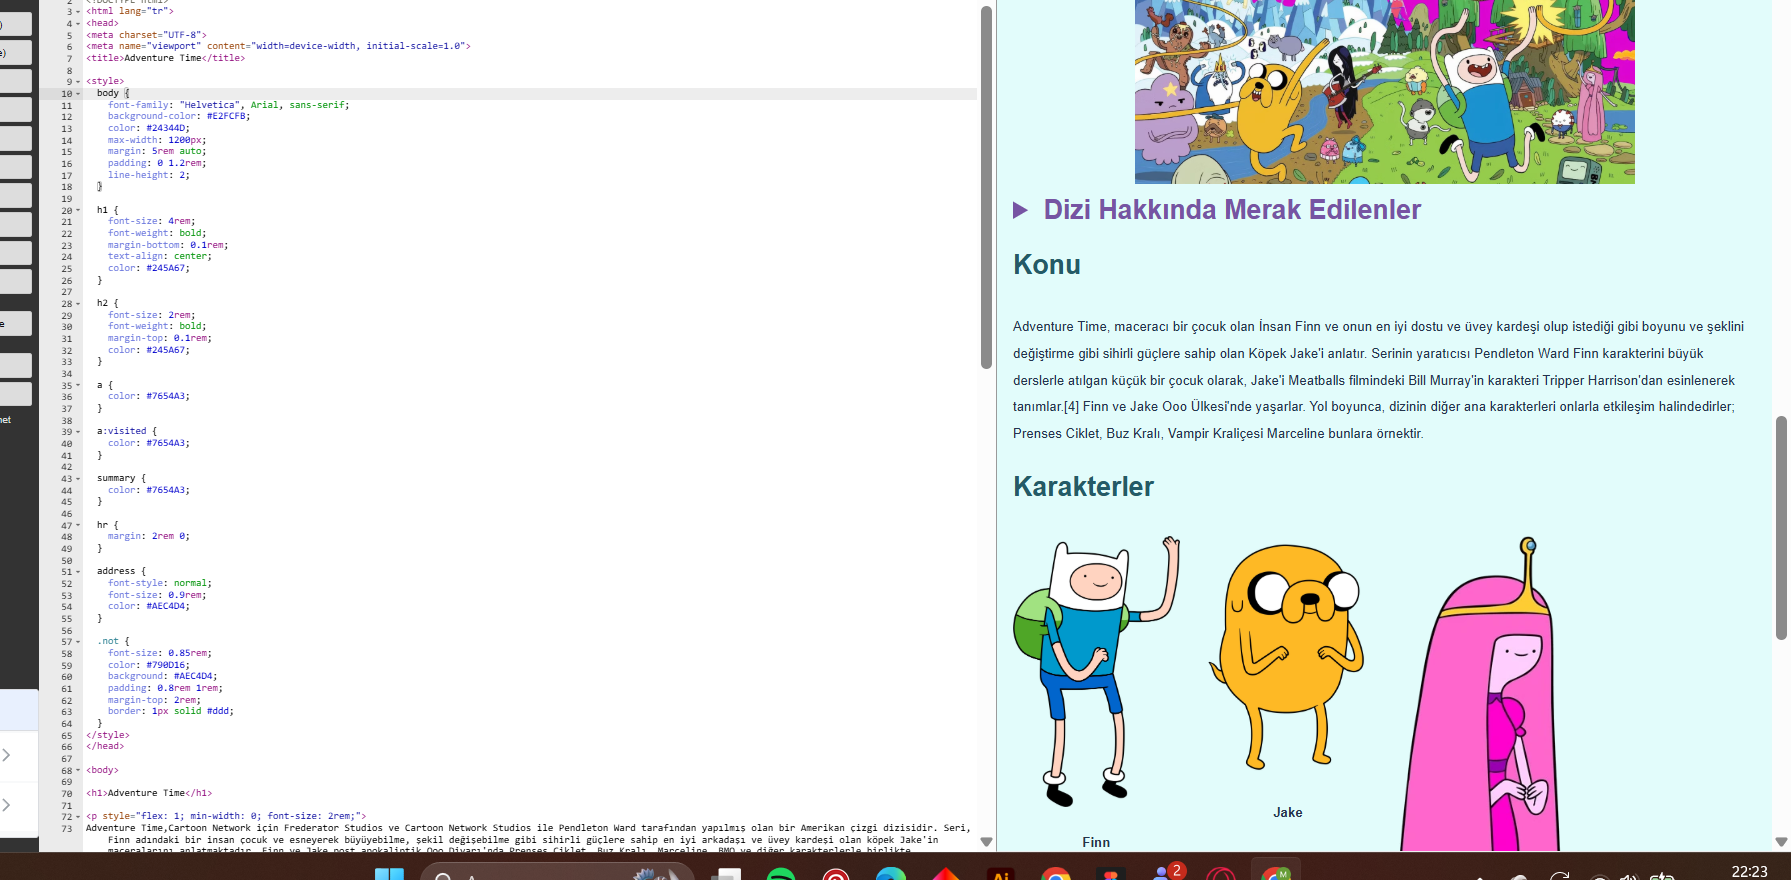
\includegraphics{hafta3b.png}}} \\
\multicolumn{3}{c}{\resizebox{14cm}{!}{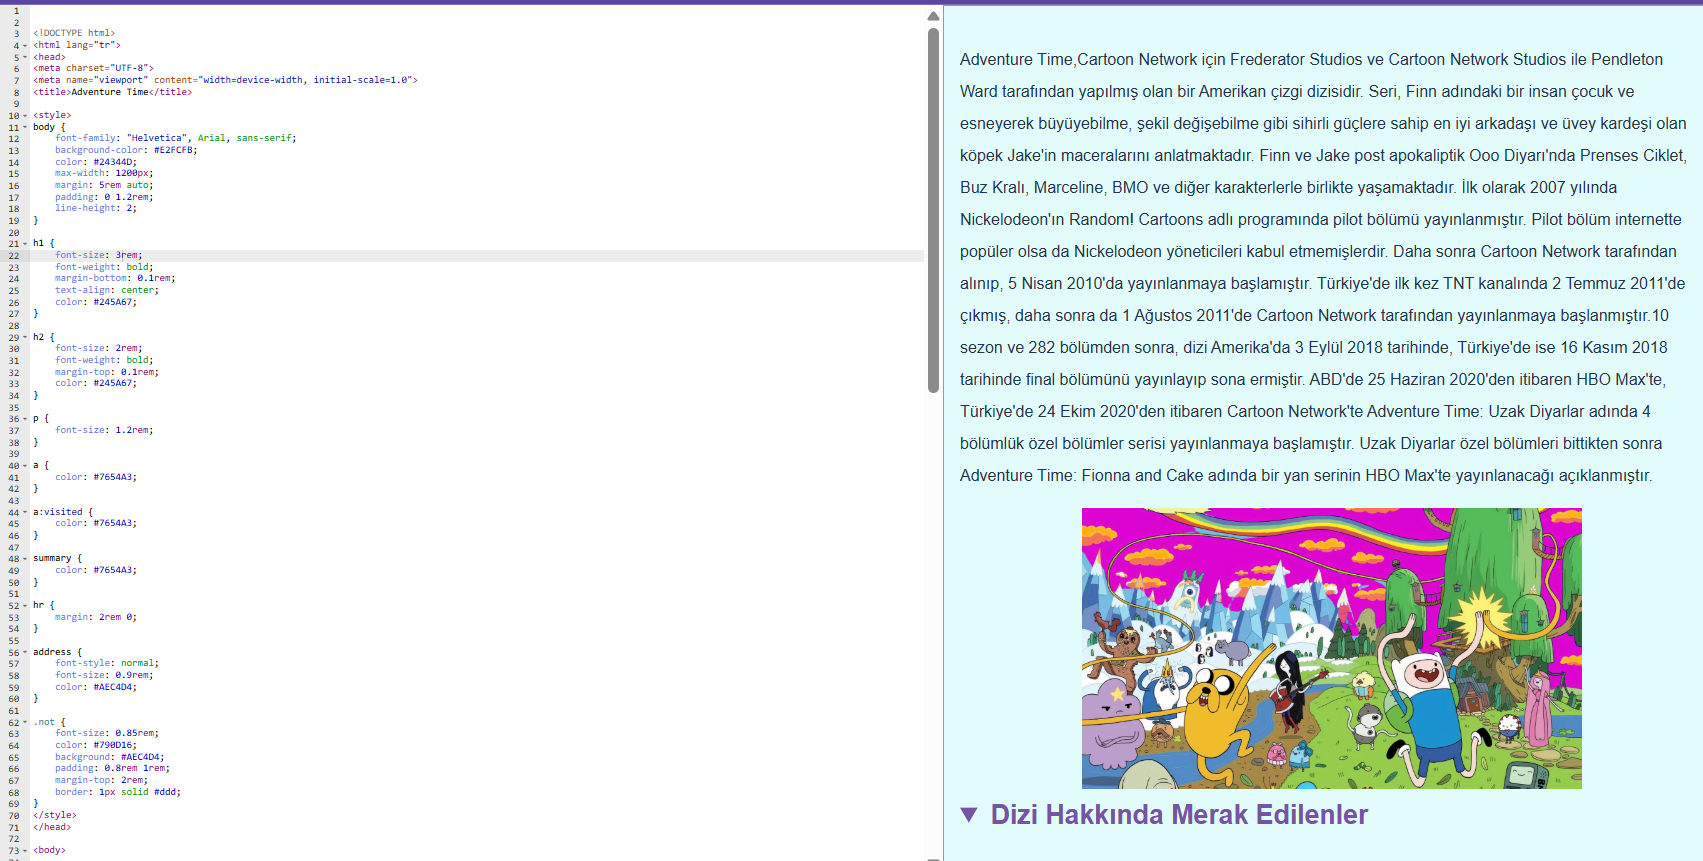
\includegraphics{hafta3c.png}}} \\
\multicolumn{3}{c}{\resizebox{14cm}{!}{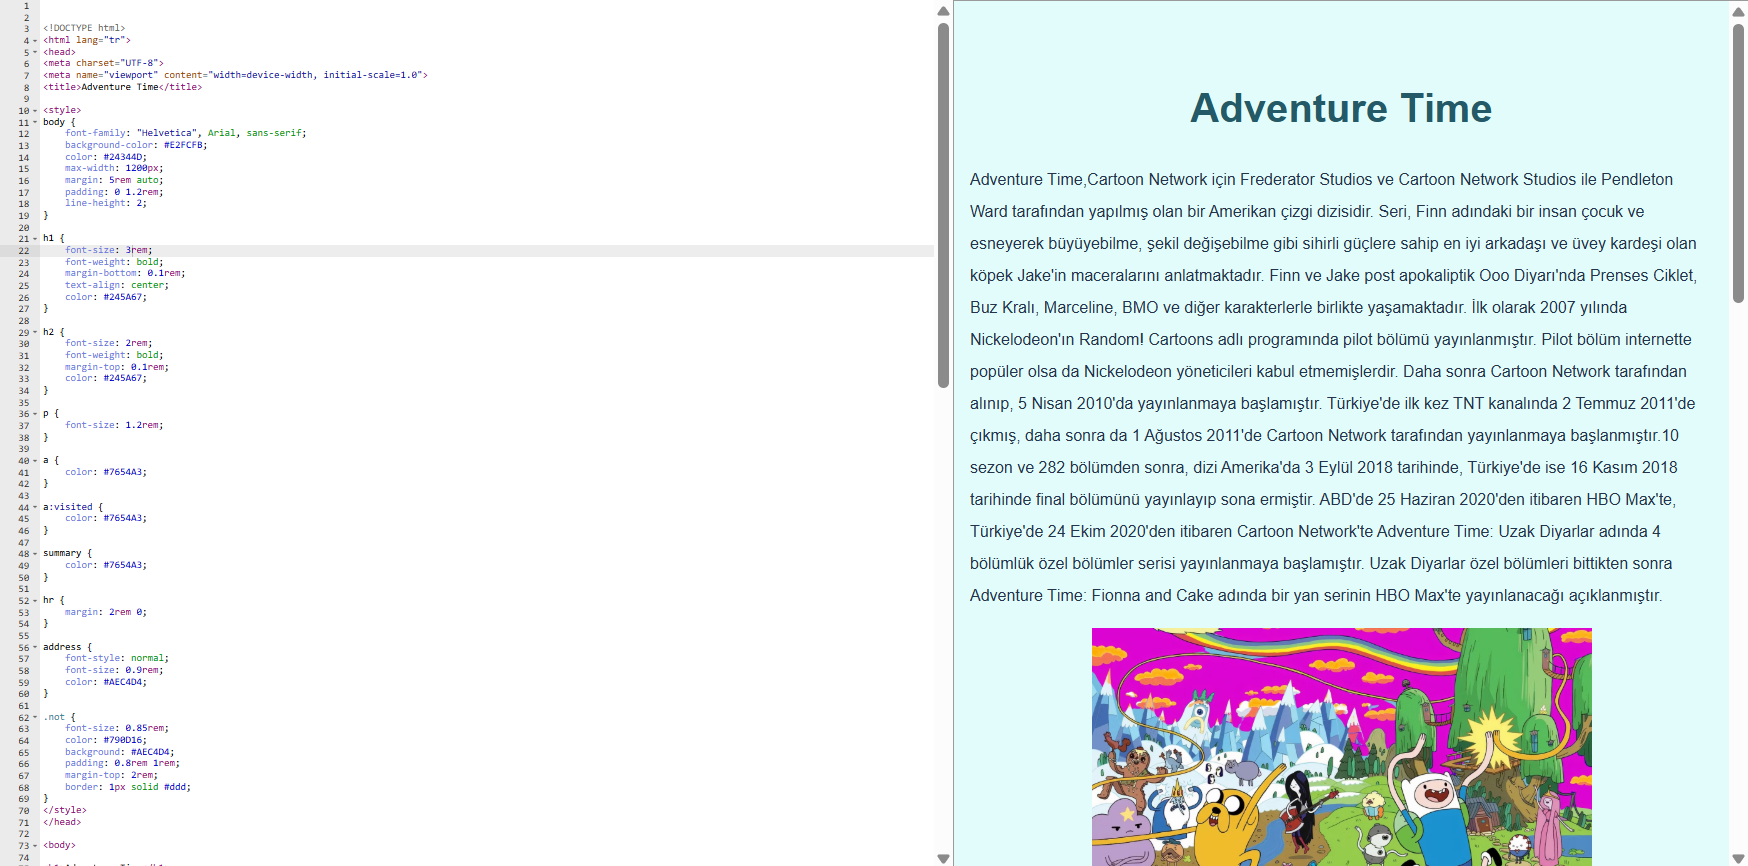
\includegraphics{hafta3d.png}}} \\
\multicolumn{3}{c}{\resizebox{14cm}{!}{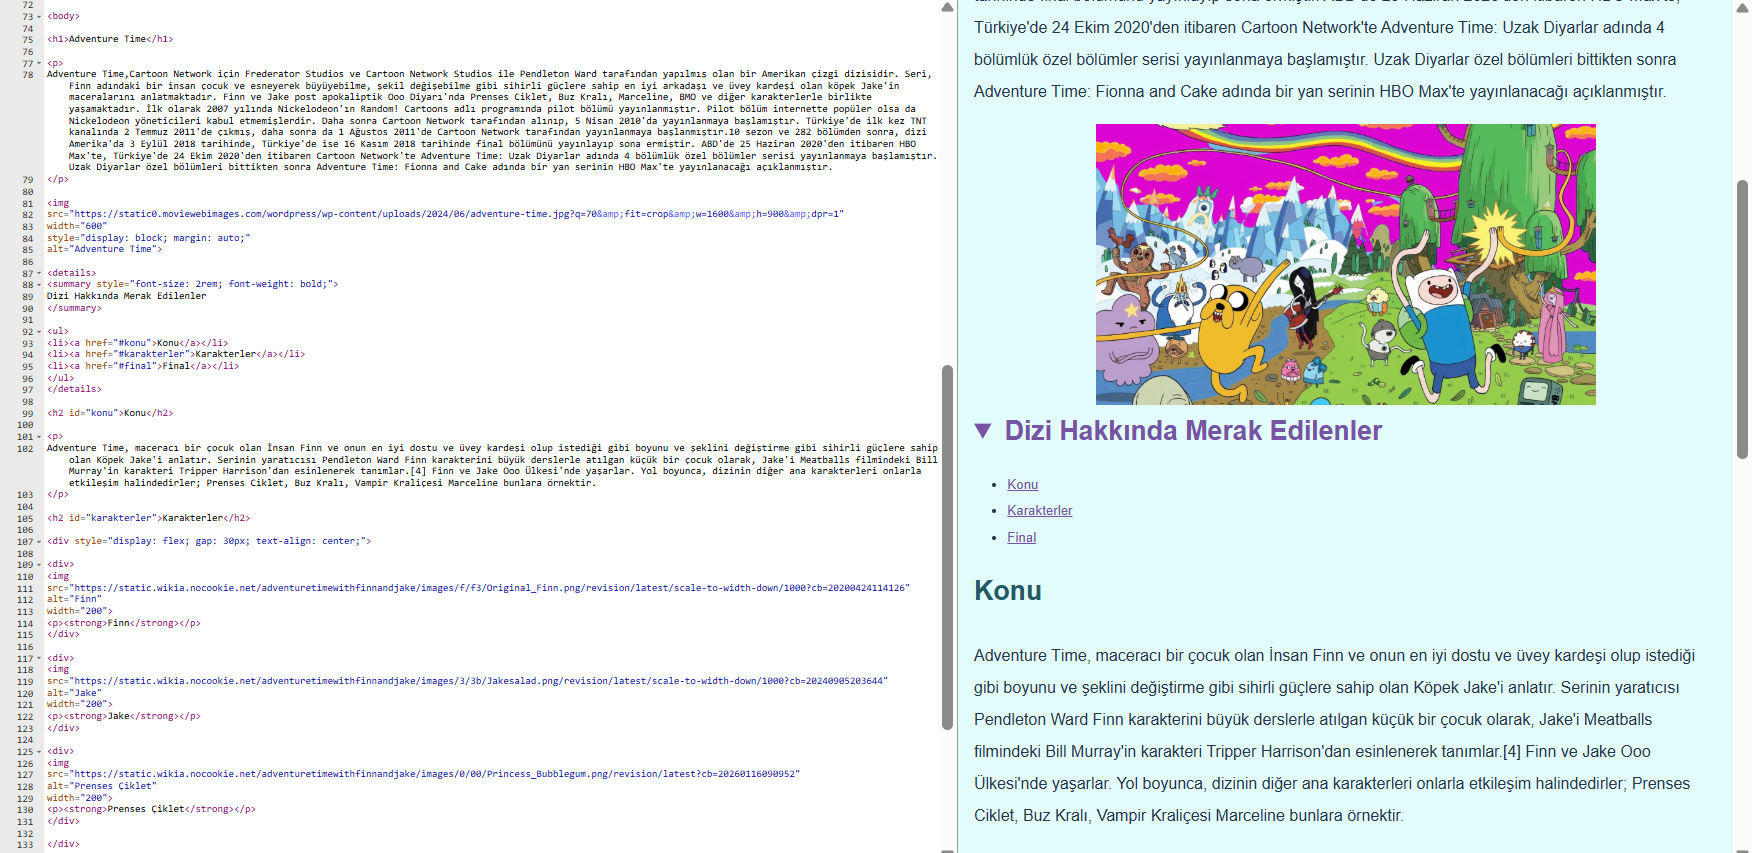
\includegraphics{hafta3e.png}}} \\
\multicolumn{3}{c}{\resizebox{14cm}{!}{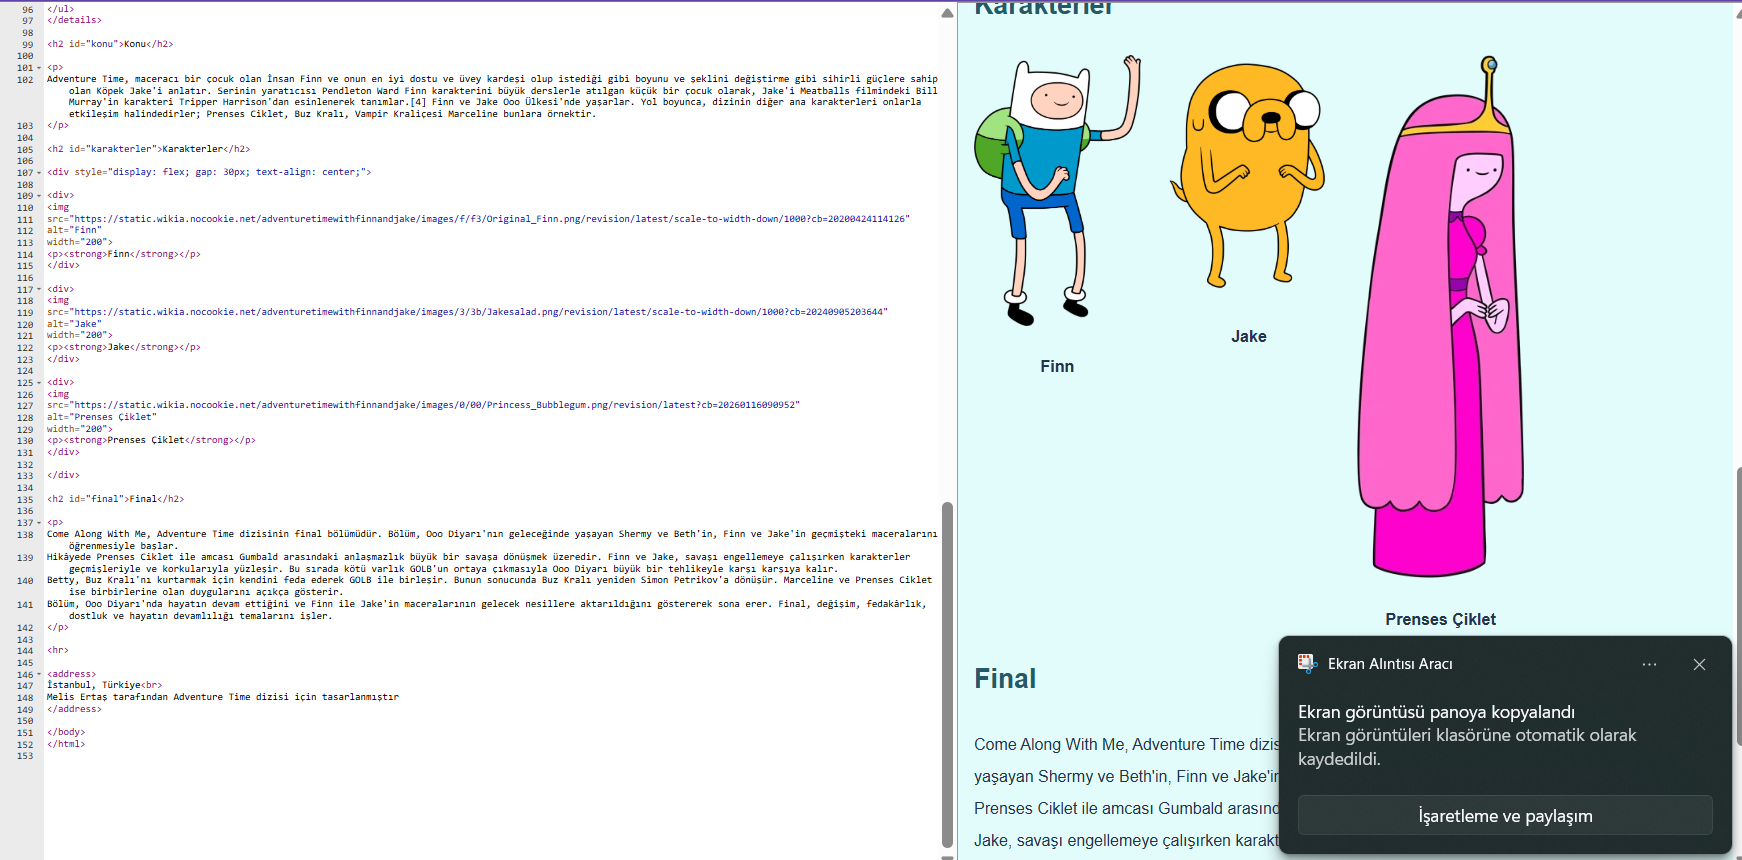
\includegraphics{hafta3f.png}}} \\
\midrule
\textbf{4. hafta}\newline [tarih] &
Bu haftayı sonradan telafi ederek tamamladım. Düğmeye basınca \texttt{textContent} ile sayfadaki yazıyı değiştiren örneği yaptım. Ad soran örnekte \texttt{input} değerini okudum, boşsa \texttt{if} ve \texttt{alert} ile uyarı verdim. Artır ve azalt düğmeleriyle \texttt{let} değişkeni kullanan bir sayaç yazdım.\newline \textbf{Commit:} 4. hafta telafi: metin degistirme, ad sorma ve sayac\par\vspace{3pt}\small $\square$ Ders içinde katılım sergiledim\par $\boxtimes$ Telafi yaptım &
Görsel aşağıda \\*
\multicolumn{3}{c}{\resizebox{14cm}{!}{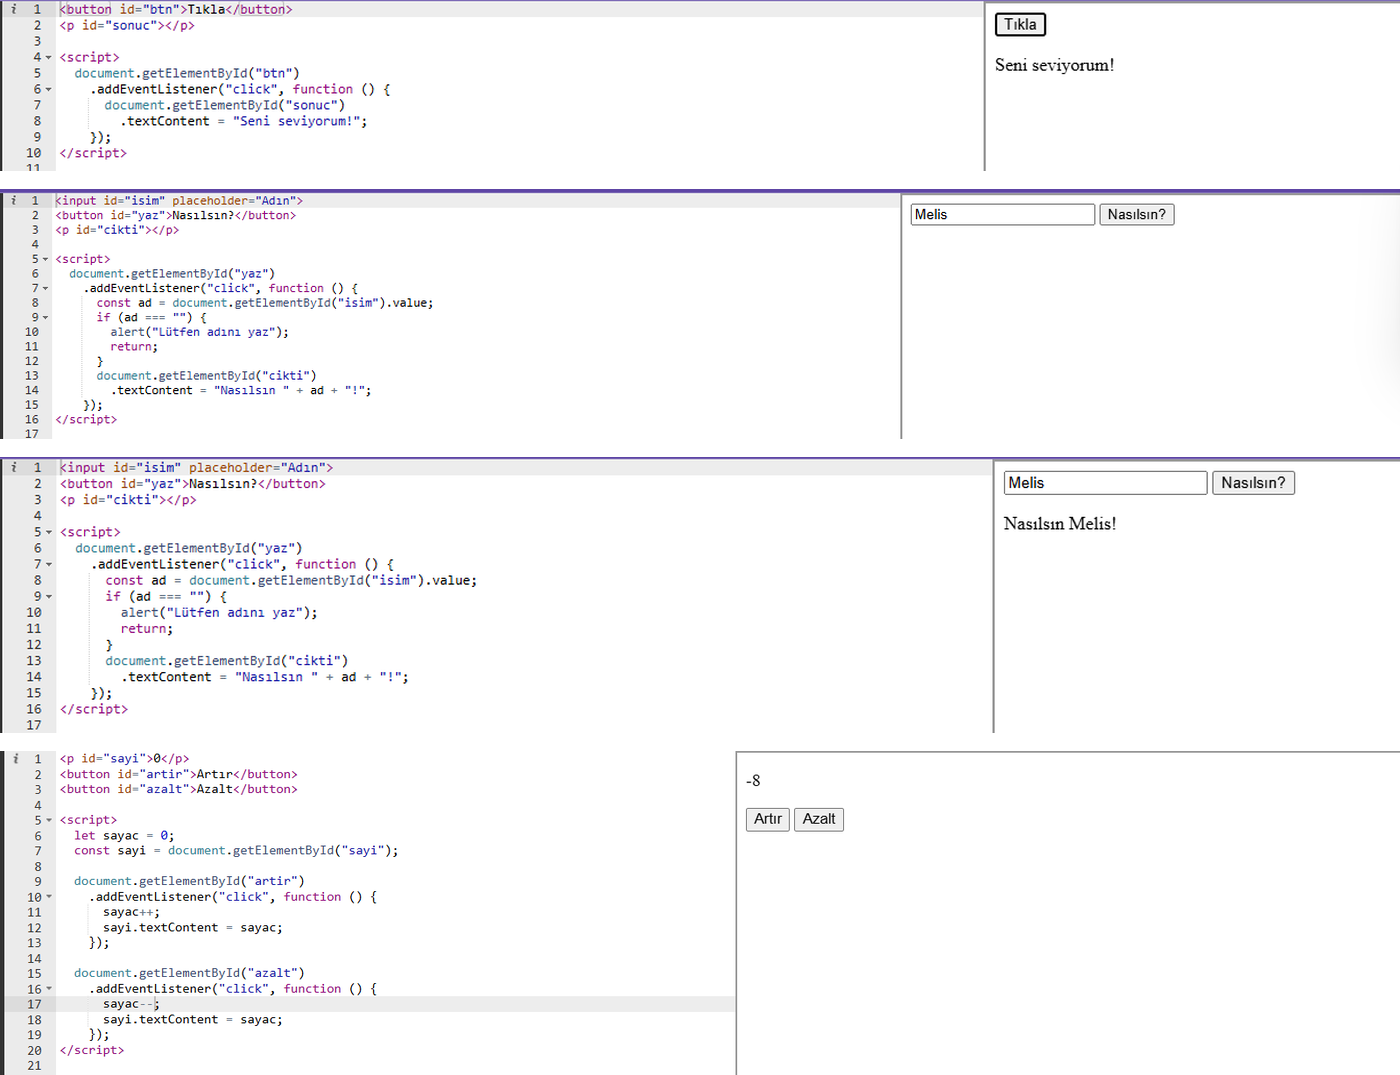
\includegraphics{hafta4.png}}} \\
\midrule
\textbf{5. hafta}\newline [tarih] &
Bu haftayı sonradan telafi ederek tamamladım. Düğmeye basınca \texttt{addEventListener} ve \texttt{window.location.href} ile siteye yönlendiren örneği yaptım. Kart eşleştirme oyununda \texttt{querySelectorAll}, \texttt{forEach}, \texttt{if-else} ve \texttt{setTimeout} kullandım; eşleşen kartlar gizleniyor, eşleşmeyenler eski rengine dönüyor.\newline \textbf{Commit:} 5. hafta telafi: yonlendirme dugmesi ve kart eslestirme oyunu\par\vspace{3pt}\small $\square$ Ders içinde katılım sergiledim\par $\boxtimes$ Telafi yaptım &
Görsel aşağıda \\*
\multicolumn{3}{c}{\resizebox{14cm}{!}{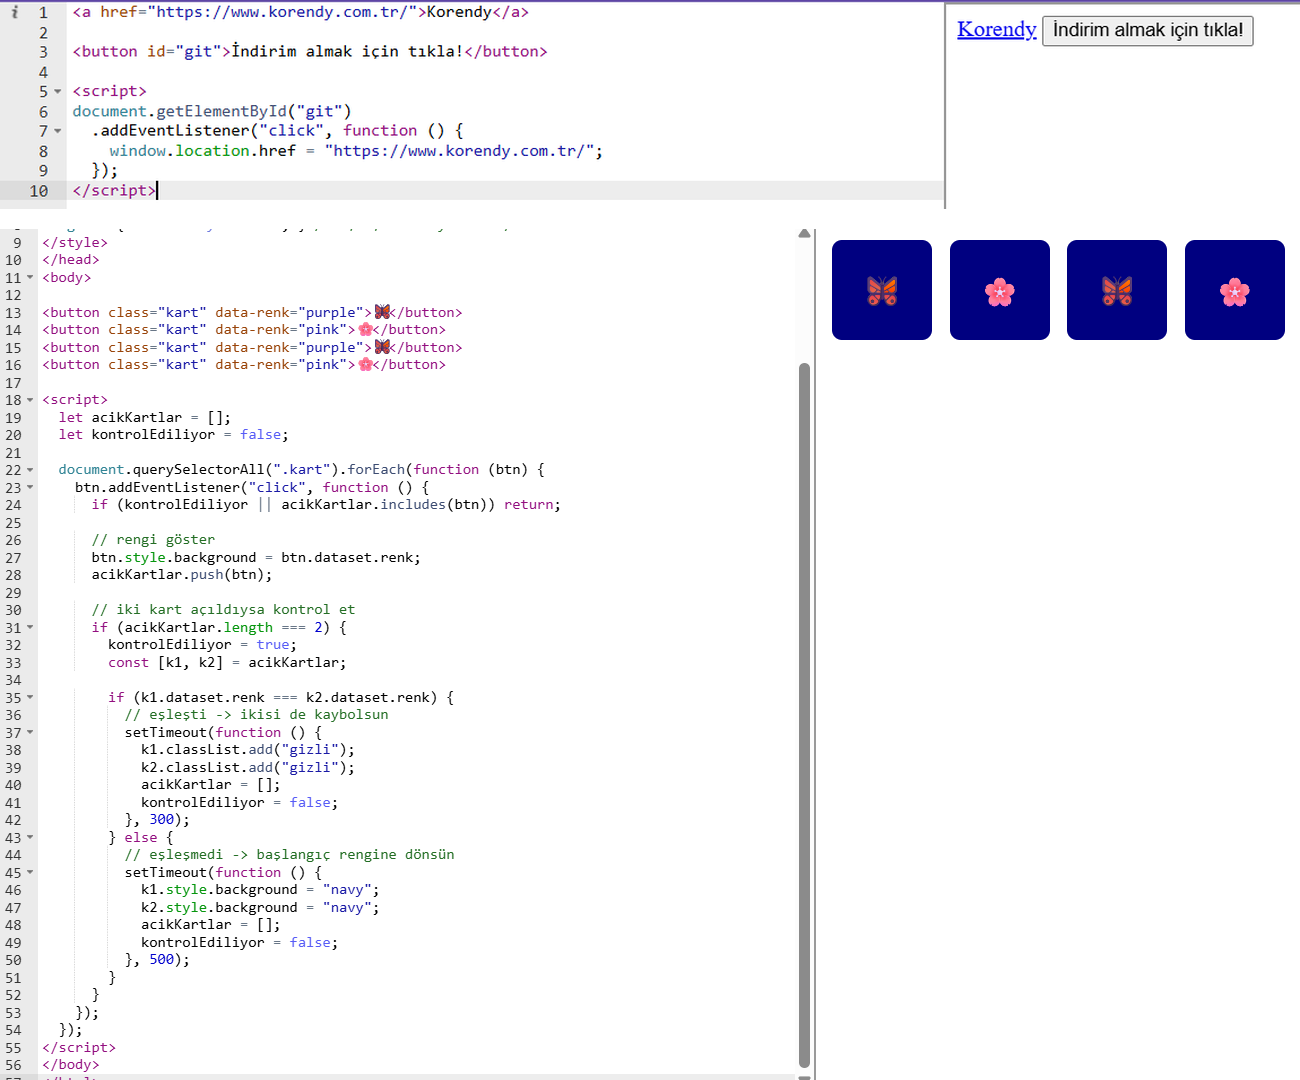
\includegraphics{hafta5.png}}} \\
\midrule
\textbf{6. hafta}\newline [tarih] &
Bu haftayı sonradan telafi ederek tamamladım. \texttt{if-else} koşul yapısını çalıştım. Düğmeye basınca kutu siyahsa kırmızı, değilse siyah yapan örneği \texttt{getElementById} ve \texttt{onclick} ile uyguladım. Harici CSS örneğinde \texttt{<link>} ile stil dosyası bağlayıp başlık ve alt bilgiyi renklendirdim.\newline \textbf{Commit:} 6. hafta telafi: if-else ve harici CSS\par\vspace{3pt}\small $\square$ Ders içinde katılım sergiledim\par $\boxtimes$ Telafi yaptım &
Görsel aşağıda \\*
\multicolumn{3}{c}{\resizebox{13cm}{!}{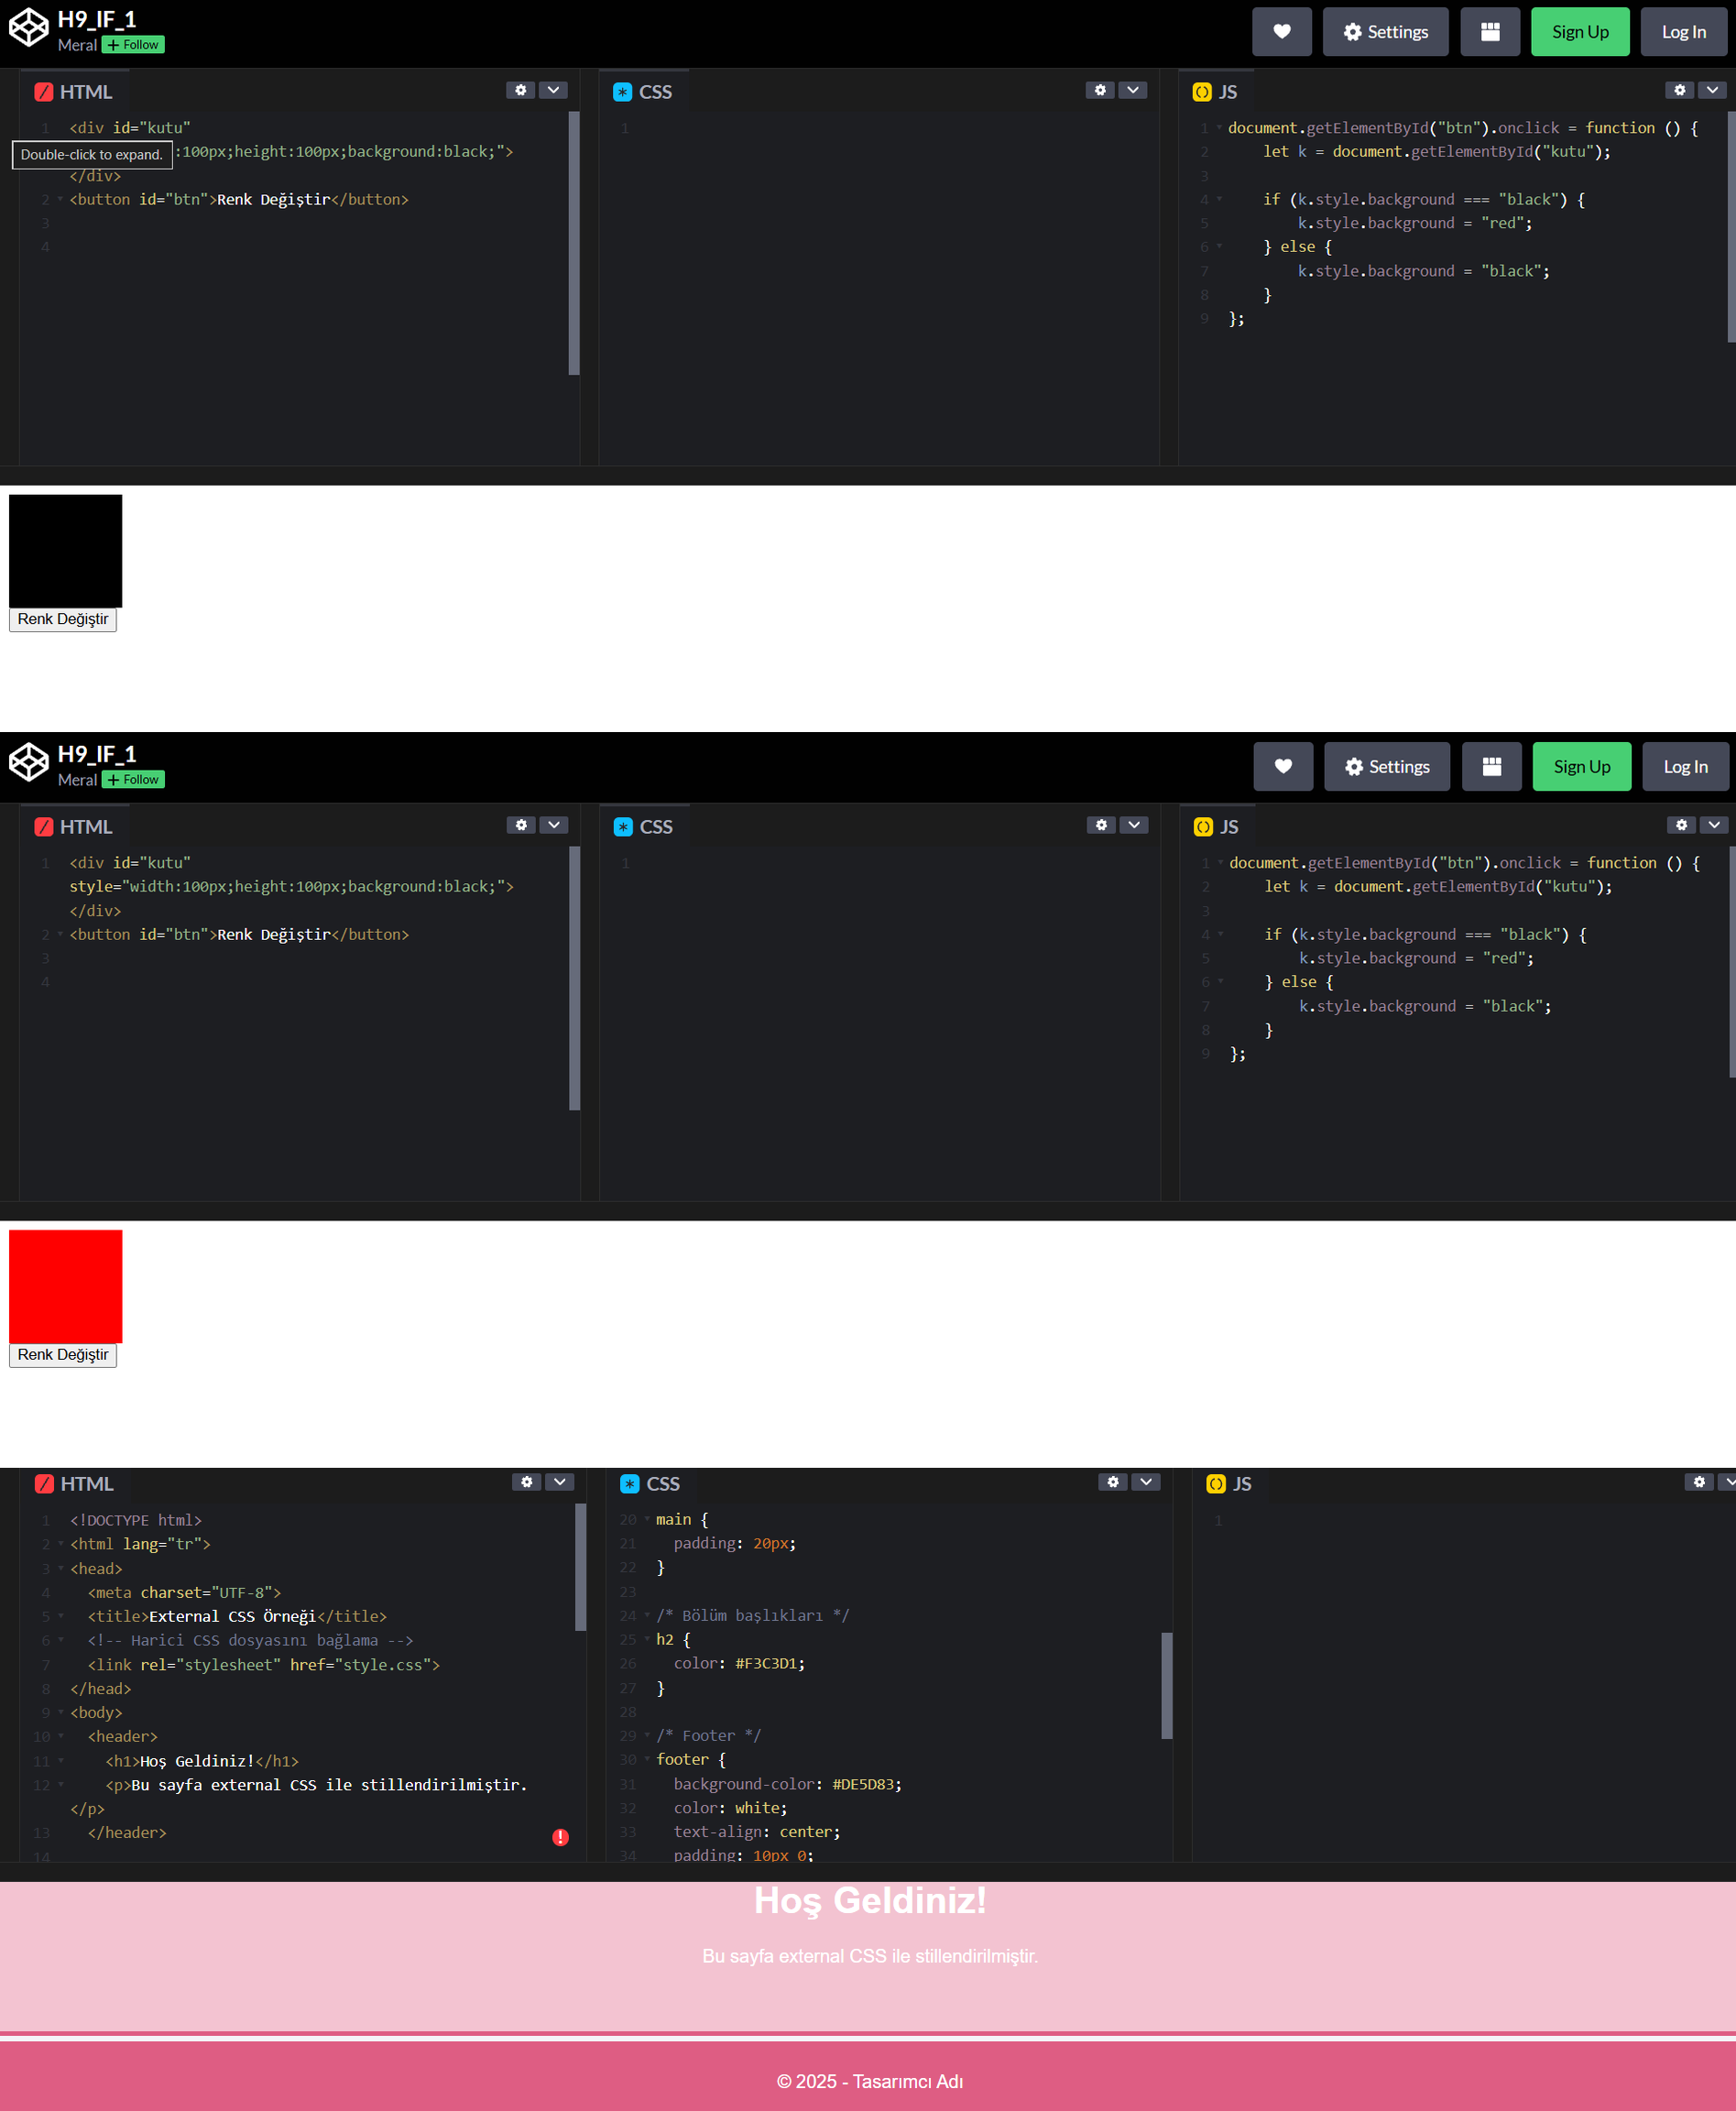
\includegraphics{hafta6.png}}} \\
\end{longtable}

% ====================================================================
\section{Test ve Değerlendirme}
% ====================================================================
\begin{center}
\rowcolors{2}{acik}{white}
\begin{tabular}{@{}p{6cm}p{3.4cm}p{3.4cm}@{}}
\toprule
\rowcolor{ana}\textcolor{white}{\textbf{Özellik}} & \textcolor{white}{\textbf{Bilgisayar}} & \textcolor{white}{\textbf{Telefon}} \\
\midrule
\relax Arama, tür filtresi ve masal geçişleri & Çalışıyor & Çalışıyor \\
\relax Favoriler ve yazı boyutu ayarı & Çalışıyor & Çalışıyor \\
\relax Menü takibi ve düzen & Çalışıyor & Çalışıyor \\
\bottomrule
\end{tabular}
\end{center}

\textbf{Denenen tarayıcılar:} Chromium. Telefon görünümü Claude ile otomatik testte iPhone SE, iPhone 13, Pixel 5 ve Galaxy S9+ benzetimleriyle denendi; yatay taşma veya işlev hatası görülmedi. Gerçek telefonda ve Safari'de deneme yapılmadı.

% ====================================================================
\section{Sunum Videosu}
% ====================================================================
\begin{center}
\begin{tabular}{@{}ll@{}}
\textbf{Video süresi:} & 10:16 \quad  \\
\textbf{Görünürlük:} & Listelenmemiş \\
\textbf{Bağlantı:} & \youtubelink \\
\end{tabular}
\end{center}

\subsection{Video Kontrol Listesi}
\begin{itemize}[label={}]
  \item $\square$ Süre 12--18 dakika aralığında.
  \item $\square$ Sunum boyunca kameram açık, yüzüm görünüyor.
  \item $\square$ Görünürlük \textbf{Listelenmemiş} (ya da Herkese açık); \textbf{Özel} değil.
  \item $\square$ Bağlantıyı gizli pencerede açtım, video oynuyor.
  \item $\square$ YouTube videoyu işlemeyi bitirdi.
  \item $\square$ Videoyu baştan sona izledim; ses ve kamera tüm sunumda var.
  \item $\boxtimes$ Kapaktaki bağlantı ile bu bölümdeki bağlantı aynı.
\end{itemize}

% ====================================================================
\section{Sonuç ve Kendi Değerlendirmem}
% ====================================================================
Bu projede sekiz Türk masalını, internet gerektirmeden çalışan tek bir HTML sayfasında topladım. Küçük alıştırmalarda öğrendiğim \texttt{addEventListener}, \texttt{if-else} ve \texttt{textContent} gibi yapıların gerçek bir sayfada nasıl birlikte çalıştığını bu projede gördüm. Arama, filtre ve favoriler bölümü, JavaScript'in sayfayı süslemekten çok kullanımı kolaylaştırdığını anlamamı sağladı. Tasarım tarafında renk, yazı tipi ve boşluk kararlarının okumayı doğrudan etkilediğini fark ettim. En çok zorlandığım konu, sayfa büyüdükçe kodun karışması ve sayfanın telefonda düzgün görünmesini sağlamak oldu. Bunu kodu bölümlere ayırarak, sayfayı farklı ekran genişliklerinde deneyerek ve yapay zekâdan destek alarak çözdüm. İleride masal sayısını on ikiye çıkarmak, gül renginin küçük yazılardaki karşıtlığını artırmak ve sayfayı gerçek telefonlarda daha çok denemek isterim.

% ====================================================================
\section{Kaynakça}
% ====================================================================
\begin{thebibliography}{9}
\bibitem{k1} T.C. Kültür Portalı. \emph{Felek}. \url{https://www.kulturportali.gov.tr/portal/felek}, erişim: 6 Kasım 2026.
\bibitem{k2} T.C. Kültür Portalı. \emph{Üç Haylaz Masalı}. \url{https://www.kulturportali.gov.tr/portal/uchaylazmasali}, erişim: 6 Kasım 2026.
\bibitem{k3} T.C. Kültür Portalı. \emph{Derviş}. \url{https://www.kulturportali.gov.tr/portal/dervis}, erişim: 6 Kasım 2026.
\bibitem{k4} T.C. Kültür Portalı. \emph{İncili Çadır}. \url{https://www.kulturportali.gov.tr/portal/incilicadir}, erişim: 6 Kasım 2026.
\bibitem{k5} T.C. Kültür Portalı. \emph{Öksüz Kız}. \url{https://www.kulturportali.gov.tr/portal/oksuzkiz}, erişim: 6 Kasım 2026.
\bibitem{k6} T.C. Kültür Portalı. \emph{Kurnaz Kurt Masalı}. \url{https://www.kulturportali.gov.tr/portal/kurnazkurtmasali}, erişim: 6 Kasım 2026.
\bibitem{k7} T.C. Kültür Portalı. \emph{Dört Öğüt}. \url{https://www.kulturportali.gov.tr/portal/dortogut-1}, erişim: 6 Kasım 2026.
\bibitem{k8} T.C. Kültür Portalı. \emph{İnatçı Horoz}. \url{https://www.kulturportali.gov.tr/portal/inatcihoruz}, erişim: 6 Kasım 2026.
\bibitem{k9} Anthropic. \emph{Claude}. \url{https://claude.ai}, 3 Kasım 2026.
\bibitem{k10} OpenAI. \emph{ChatGPT}. \url{https://chatgpt.com}, giriş görseli ve masal kapaklarının üretimi için kullanıldı.
\end{thebibliography}

% ====================================================================
\appendix
\section{Teslim Kontrol Listesi}
% ====================================================================
\begin{itemize}[label={}]
  \item $\square$ MEBİS'e \textbf{yalnızca bu raporun PDF'ini} yükleyeceğim. ZIP ve HTML dosyası yüklemeyeceğim.
  \item $\boxtimes$ PDF dosya adı \texttt{OgrenciNo\_AdSoyad\_vize.pdf} biçiminde.
  \item $\square$ Kapaktaki GitHub ve YouTube bağlantıları doğru; PDF'te tıklayıp denedim.
  \item $\boxtimes$ GitHub deposunda web sayfası (tek \texttt{.html}), rapor PDF'i, \texttt{.tex} kaynakları ve \texttt{README.md} var.
  \item $\boxtimes$ GitHub deposu \textbf{herkese açık} (ya da öğretim üyesine erişim verdim).
  \item $\square$ Çalışmamın son hâli teslim saatinden \textbf{önce} depoya gönderildi (sonraki commitler değerlendirilmez).
  \item $\boxtimes$ Sayfa içsel CSS ve içsel JavaScript kullanıyor, harici dosya gerektirmiyor.
  \item $\square$ Hazır taslak kullanmadım; yapay zekâ kullandıysam Bölüm 5'i doldurdum.
  \item $\square$ Çalışmanın mantığını sunumda anlatabilirim.
\end{itemize}

\end{document}